% mnras_template.tex 
%
% LaTeX template for creating an MNRAS paper
%
% v3.2 released 20 July 2023
% (version numbers match those of mnras.cls)
%
% Copyright (C) Royal Astronomical Society 2015
% Authors:
% Keith T. Smith (Royal Astronomical Society)

%%%%%%%%%%%%%%%%%%%%%%%%%%%%%%%%%%%%%%%%%%%%%%%%%%%%%%%%%%%%%%%%%%%%%%%%%%%%%%%%%%%%%%%%%%%%%%%%%%%%
% Basic setup. Most papers should leave these options alone.
\documentclass[fleqn,usenatbib]{mnras}

% MNRAS is set in Times font. If you don't have this installed (most LaTeX
% installations will be fine) or prefer the old Computer Modern fonts, comment
% out the following line
\usepackage{newtxtext,newtxmath}
% Depending on your LaTeX fonts installation, you might get better results with one of these:
%\usepackage{mathptmx}
%\usepackage{txfonts}

% Use vector fonts, so it zooms properly in on-screen viewing software
% Don't change these lines unless you know what you are doing
\usepackage[T1]{fontenc}

% Allow "Thomas van Noord" and "Simon de Laguarde" and alike to be sorted by "N" and "L" etc. in the bibliography.
% Write the name in the bibliography as "\VAN{Noord}{Van}{van} Noord, Thomas"
\DeclareRobustCommand{\VAN}[3]{#2}
\let\VANthebibliography\thebibliography
\def\thebibliography{\DeclareRobustCommand{\VAN}[3]{##3}\VANthebibliography}


%%%%% AUTHORS - PLACE YOUR OWN PACKAGES HERE %%%%%

% Only include extra packages if you really need them. Avoid using amssymb if newtxmath is enabled, as these packages can cause conflicts. newtxmatch covers the same math symbols while producing a consistent Times New Roman font. Common packages are:
\usepackage{graphicx}	
\usepackage{amsmath}	
\usepackage{physics}
\usepackage{lmodern}
\usepackage{anyfontsize}


%%%%%%%%%%%%%%%%%%%%%%%%%%%%%%%%%%%%%%%%%%%%%%%%%%%%%%%%%%%%%%%%%%%%%%%%%%%%%%%%%%%%%%%%%%%%%%%%%%%%

%%%%% AUTHORS - PLACE YOUR OWN COMMANDS HERE %%%%%

% Please keep new commands to a minimum, and use \newcommand not \def to avoid
% overwriting existing commands. Example:
%\newcommand{\pcm}{\,cm$^{-2}$}	% per cm-squared

\graphicspath{{images/}}

%%%%%%%%%%%%%%%%%%%%%%%%%%%%%%%%%%%%%%%%%%%%%%%%%%%%%%%%%%%%%%%%%%%%%%%%%%%%%%%%%%%%%%%%%%%%%%%%%%%%


%%%%%%%%%%%%%%%%%%% TITLE PAGE %%%%%%%%%%%%%%%%%%%%%%%%%%%%%%%%%%%%%%%%%%%%%%%%%%%%%%%%%%%%%%%%%%%%%

% Title of the paper, and the short title which is used in the headers.
% Keep the title short and informative.
\title[Short title, max. 45 characters]{Study of the star formation rate bimodality in SDSS galaxies at low redshift}

% The list of authors, and the short list which is used in the headers.
% If you need two or more lines of authors, add an extra line using \newauthor
\author[M. Bianchi]{
Marco Bianchi
\\
% List of institutions
University of Milano-Bicocca, Physics Department, Astrophysics and Space Physics master degree\\
Laboratory of Data Analysis 2023-2024, group 5: M. Bellotti, M. Bianchi, L. Carbone, and F. Leto Di Priolo
}

% Enter the current year, for the copyright statements etc.
\pubyear{2024}

% Don't change these lines
\begin{document}
\label{firstpage}
\pagerange{\pageref{firstpage}--\pageref{lastpage}}
\maketitle

% Abstract of the paper
\begin{abstract}
Galaxies at low redshift ($z<0.08$ for the data used here) display a bimodality in their specific star formation rate (sSFR). This phenomenon is related to several factors, including (1) the accretion processes that drive galaxy growth, (2) the feedback processes that eject gas from galaxies, and (3) the interactions between galaxies and their surrounding environment. These processes are strongly influenced by key physical properties of galaxies, such as gas mass, stellar mass, and age. Therefore, it is possible to build models that describe the time evolution of sSFR based on these simple quantities. \\
We developed two very simple analytical models, based on strong assumptions, and applied them to a subset of the Sloan Digital Sky Survey (SDSS) dataset. Our findings indicate that young, actively star-forming galaxies can be described by an open-box model, while old, passive galaxies are better represented by a closed-box model, which does not exchange gas with the surrounding halo. We also relaxed some assumptions, such as redshift-independent gas accretion, by numerically integrating the differential equation of the open-box model over infinitesimal time steps, obtaining similar results.
\bigskip
\end{abstract} 
%%%%%%%%%%%%%%%%%%%%%%%%%%%%%%%%%%%%%%%%%%%%%%%%%%%%%%%%%%%%%%%%%%%%%%%%%%%%%%%%%%%%%%%%%%%%%%%%%%%%




%%%%%%%%%%%%%%%%% BODY OF PAPER %%%%%%%%%%%%%%%%%%%%%%%%%%%%%%%%%%%%%%%%%%%%%%%%%%%%%%%%%%%%%%%%%%%%

\section{Introduction}\label{sec:introduction}
Galaxies are the fundamental building blocks of the universe at cosmological scales. Therefore, understanding how they form, evolve over time, and interact to create complex structures is crucial for advancing our knowledge about the universe and its evolution. However, capturing the extreme diversity of galaxies within a mathematical model is a very challenging task.

In this context, it is well known \citep[e.g.,][]{Kauffmann_2003} that two main populations can be identified in the plane of \textbf{specific star formation rate} (sSFR) versus \textbf{stellar mass} ($M_{\text{star}}$): one of young, actively star-forming galaxies (the \textit{main sequence}) and the other of old, mostly passive galaxies, as shown in Fig.~\ref{fig:mass_sSFR}. For this reason, a model that relates sSFR and $M_{\text{star}}$ should have at least two regimes, with a sharp transition past some threshold. In this work, we investigate the processes that either stimulate or quench the formation of new stars within galaxies at low redshift, and we try to develop simple mathematical models to test our assumptions.

The raw material for star formation is gas, which, under appropriate conditions, can collapse and form virialized objects. The amount of gas within a galaxy is not constant and is subject to a myriad of processes that depend on the main physical properties of the galaxy, such as age and mass. Therefore, we expect sSFR to drop whenever the consumed gas is no longer replaced by new gas, coming either from stars (winds, supernovae) or from outside the galaxy. 

In particular, gas inflow is strongly related to the properties of the dark matter halo that hosts the galaxy. This halo accretes matter at a certain rate from the intergalactic medium, a fraction $f_{\text{gas}}$ of which is gas, typically at very high temperatures. Such hot gas has a very strong pressure support which prevents it from accreting onto the galaxy. Therefore, the gas must cool before infall is allowed, i.e., the condition $\tau_{\text{cooling}} < \tau_{\text{free-fall}}$ is required, which can be turned into a condition on halo mass (for details check chapter 8.4 of \citet{galaxy_formation_and_evolution_2010}). We assume:
\begin{equation}
    M_{\text{halo}} \in \qty{M_{\text{halo,min}}=10^9 M_\odot \, , \, M_{\text{halo,max}}=10^{11.6} M_\odot}
	\label{eq:halo_mass_minmax}
\end{equation}


\begin{figure}
	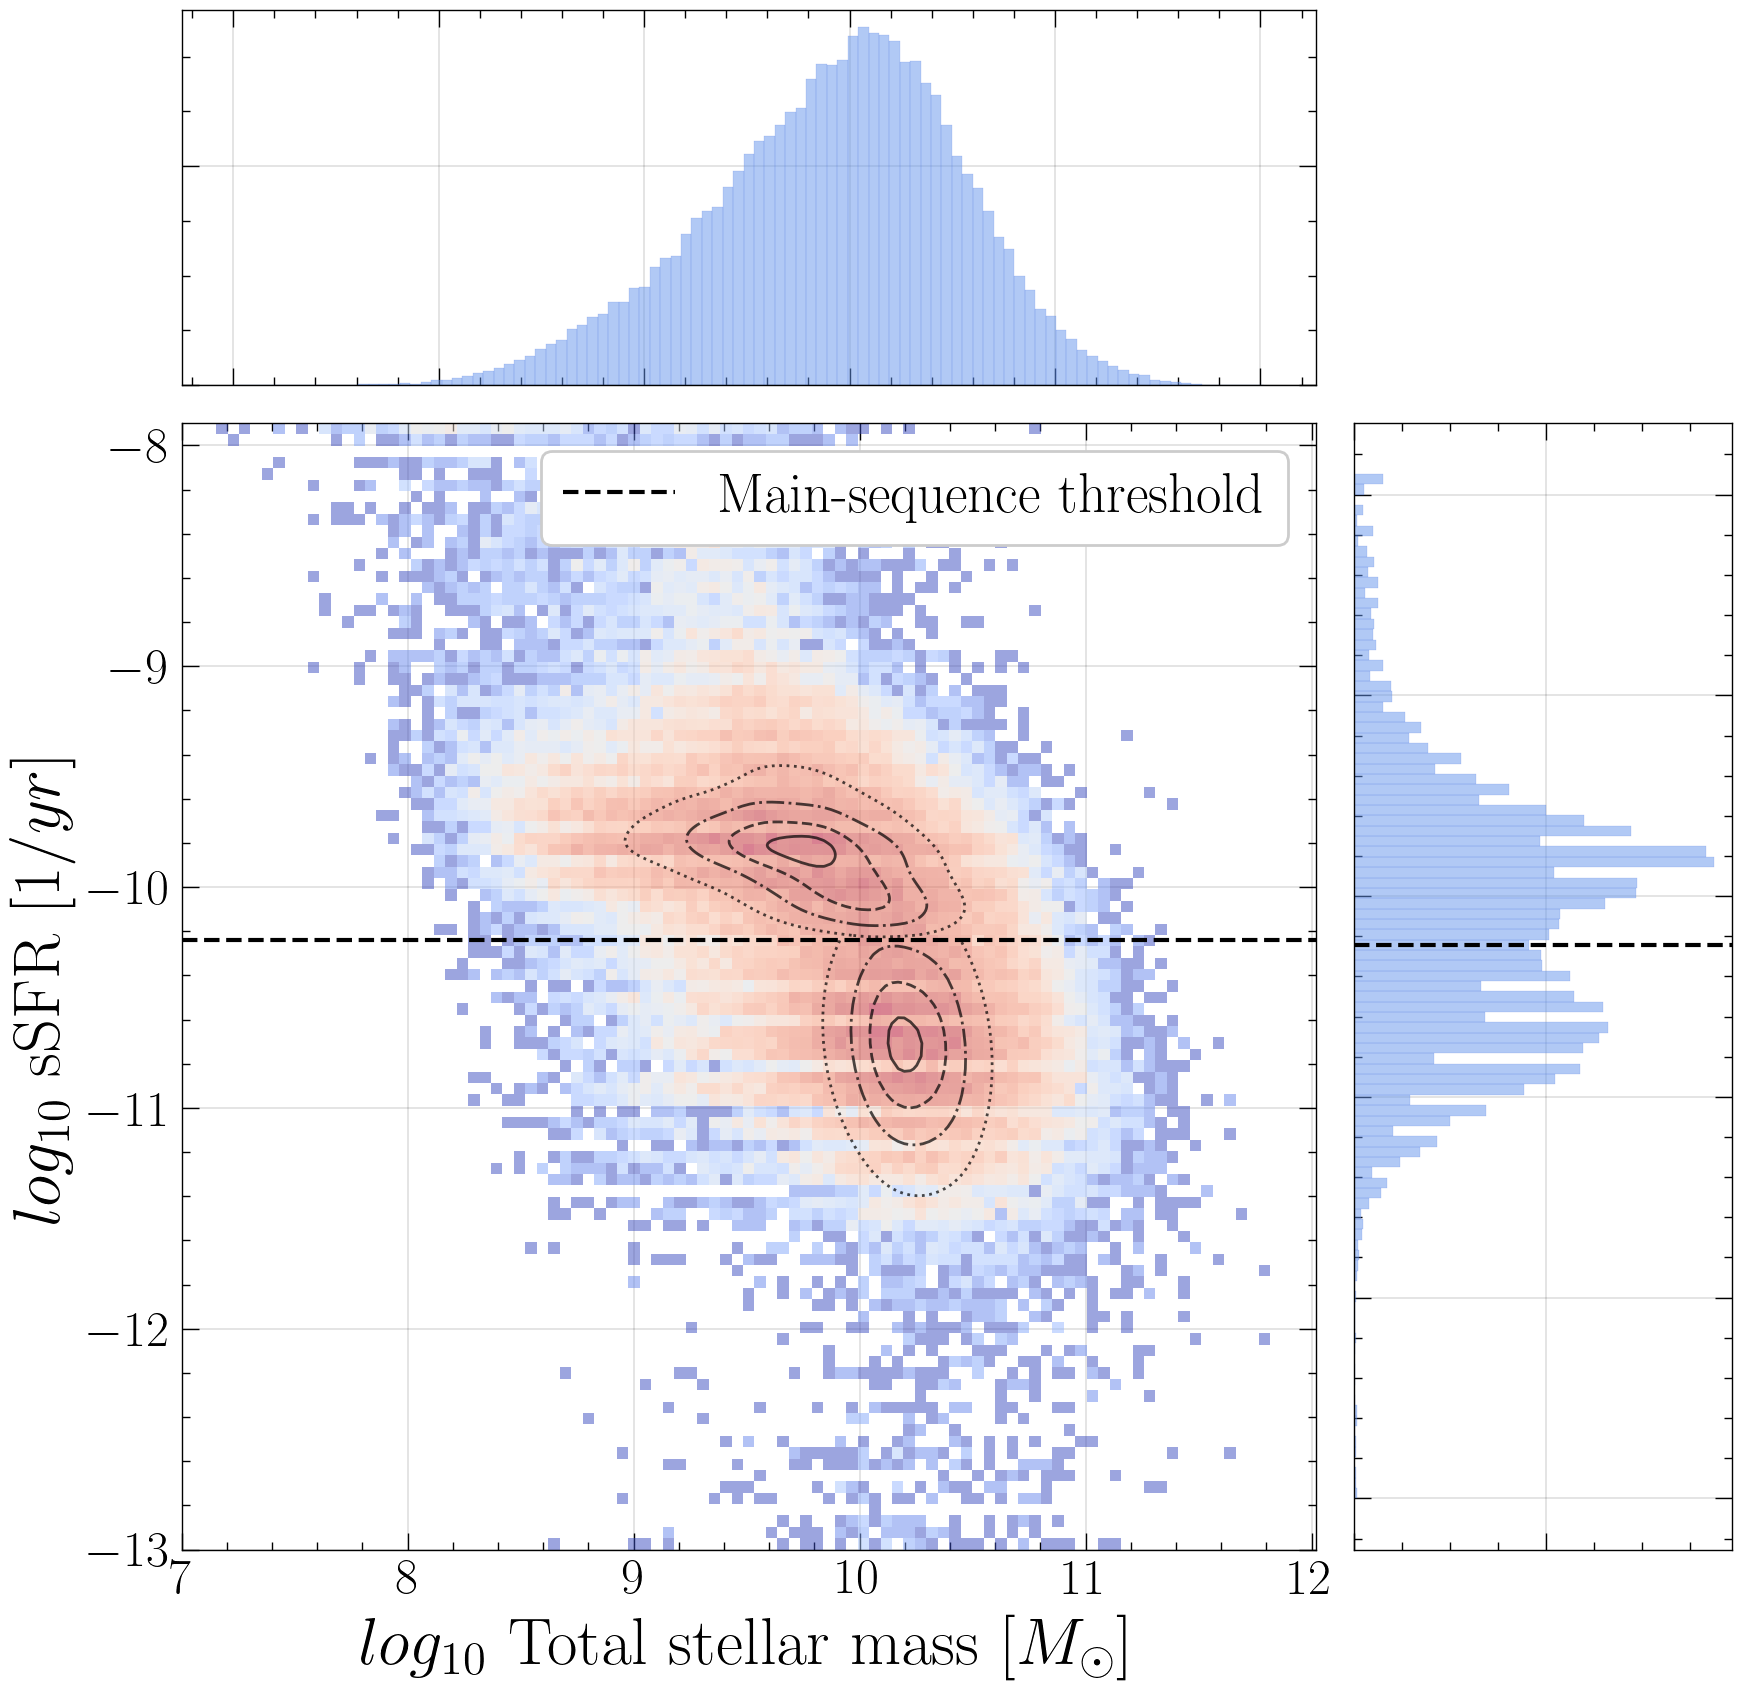
\includegraphics[width=\columnwidth]{mass_sSFR.png}
    \caption{The main panel shows a 2D histogram of sSFR versus $M_{\text{star}}$ for our dataset. The side panels display the marginal distributions of the two axes. The black dashed line indicates the value where the sSFR distribution has a local minimum, which is used to separate the main sequence from quiescent galaxies. The 25, 50, 75, and 95\% contours of both populations are shown.}
    \label{fig:mass_sSFR}
\end{figure}
%%%%%%%%%%%%%%%%%%%%%%%%%%%%%%%%%%%%%%%%%%%%%%%%%%



\section{Methods}\label{sec:methods}
This work is based on a subset of the \textbf{Sloan Digital Sky Survey} (SDSS). In particular, we study $92483$ galaxies with redshift $< 0.08$ ($z_{\text{mean}} \simeq 0.054$), for which we have five-band photometric data. This can be used to estimate the SFR

\begin{equation}
    x=\frac{-b\pm\sqrt{b^2-4ac}}{2a}.
	\label{eq:quadratic}
\end{equation}

Refer back to them as e.g. equation~(\ref{eq:quadratic}).
%%%%%%%%%%%%%%%%%%%%%%%%%%%%%%%%%%%%%%%%%%%%%%%%%%



\section{Results}\label{sec:results}
\begin{figure}
	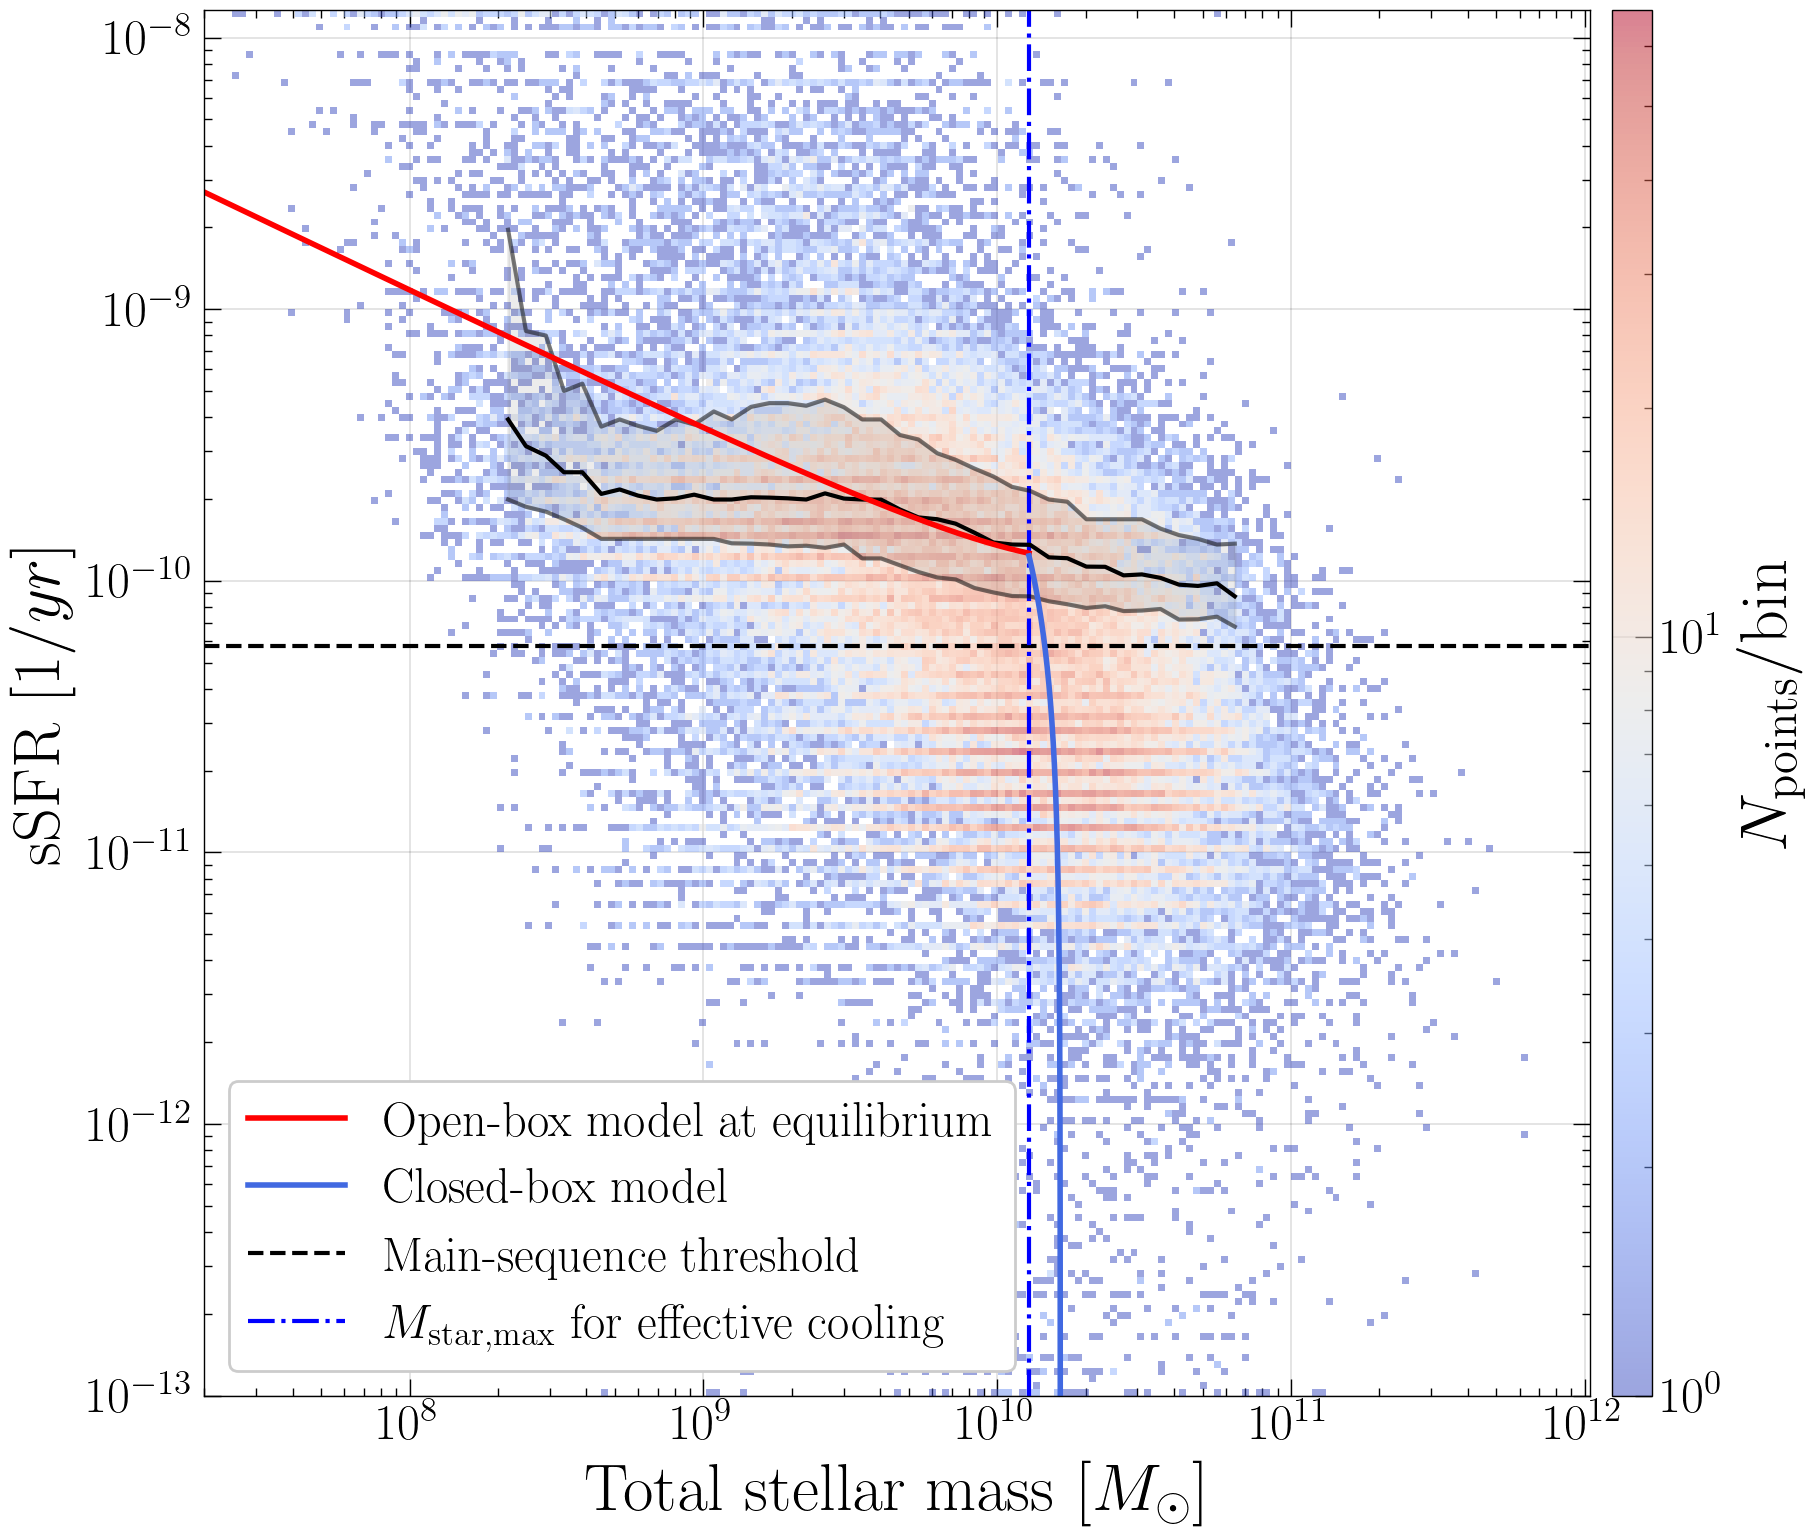
\includegraphics[width=\columnwidth]{openbox_and_closedbox.png}
    \caption{The main panel shows a 2D histogram of sSFR versus $M_{\text{star}}$ for our dataset. The side panels display the marginal distributions of the two axes. The black dashed line indicates the value where the sSFR distribution has a local minimum, which is used to separate the main sequence from quiescent galaxies. The 2D Gaussian contours of the two populations are also shown.}
    \label{fig:openbox_and_closedbox}
\end{figure}

\begin{figure}
	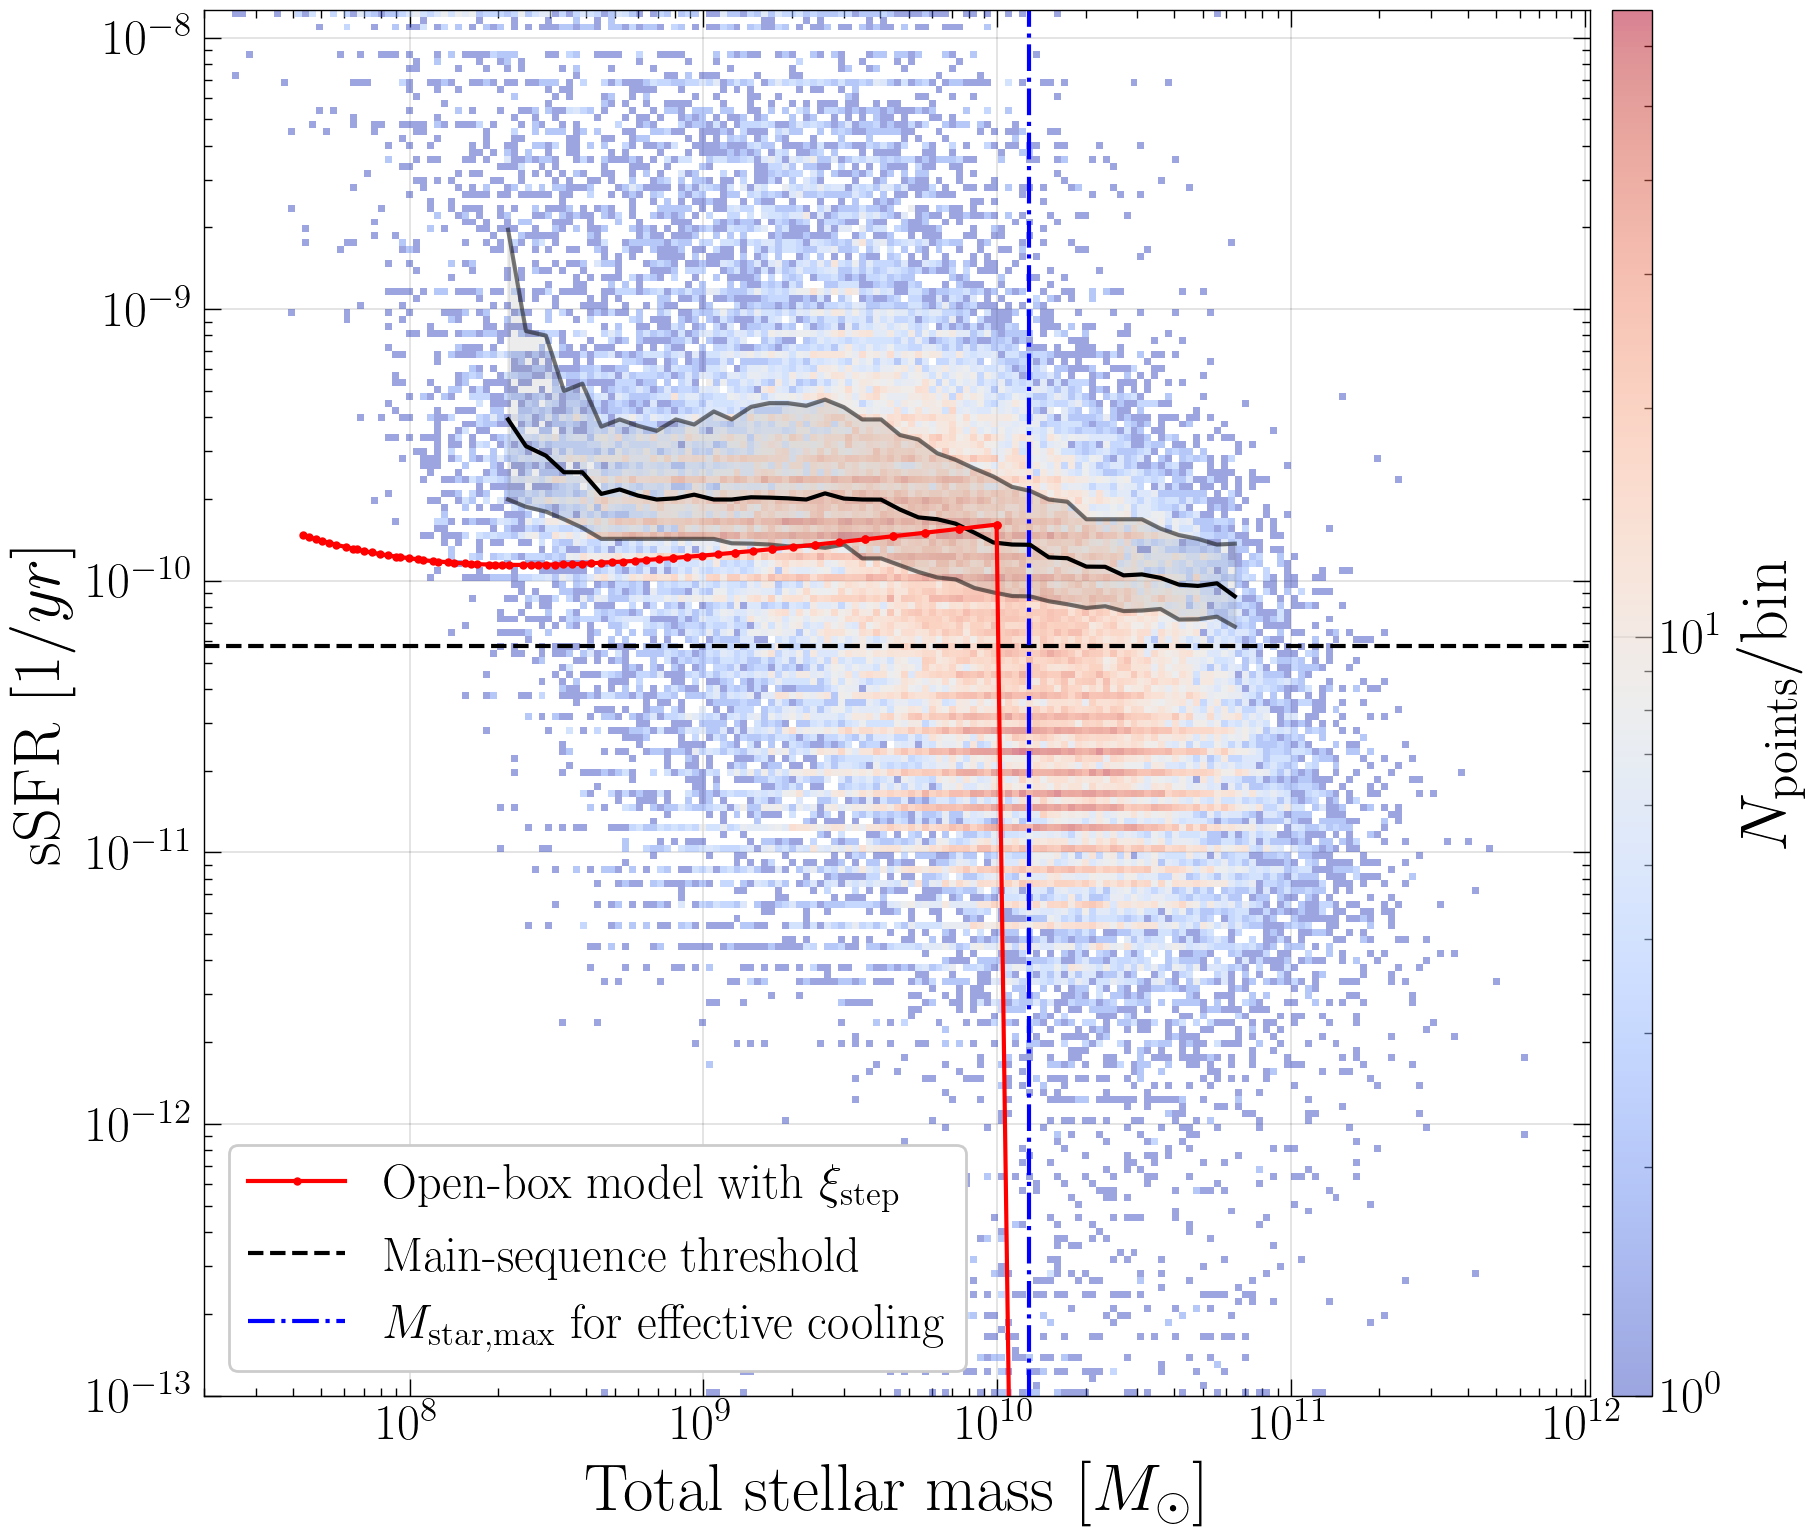
\includegraphics[width=\columnwidth]{openbox_step.png}
    \caption{The main panel shows a 2D histogram of sSFR versus $M_{\text{star}}$ for our dataset. The side panels display the marginal distributions of the two axes. The black dashed line indicates the value where the sSFR distribution has a local minimum, which is used to separate the main sequence from quiescent galaxies. The 2D Gaussian contours of the two populations are also shown.}
    \label{fig:openbox_step}
\end{figure}

\begin{figure}
	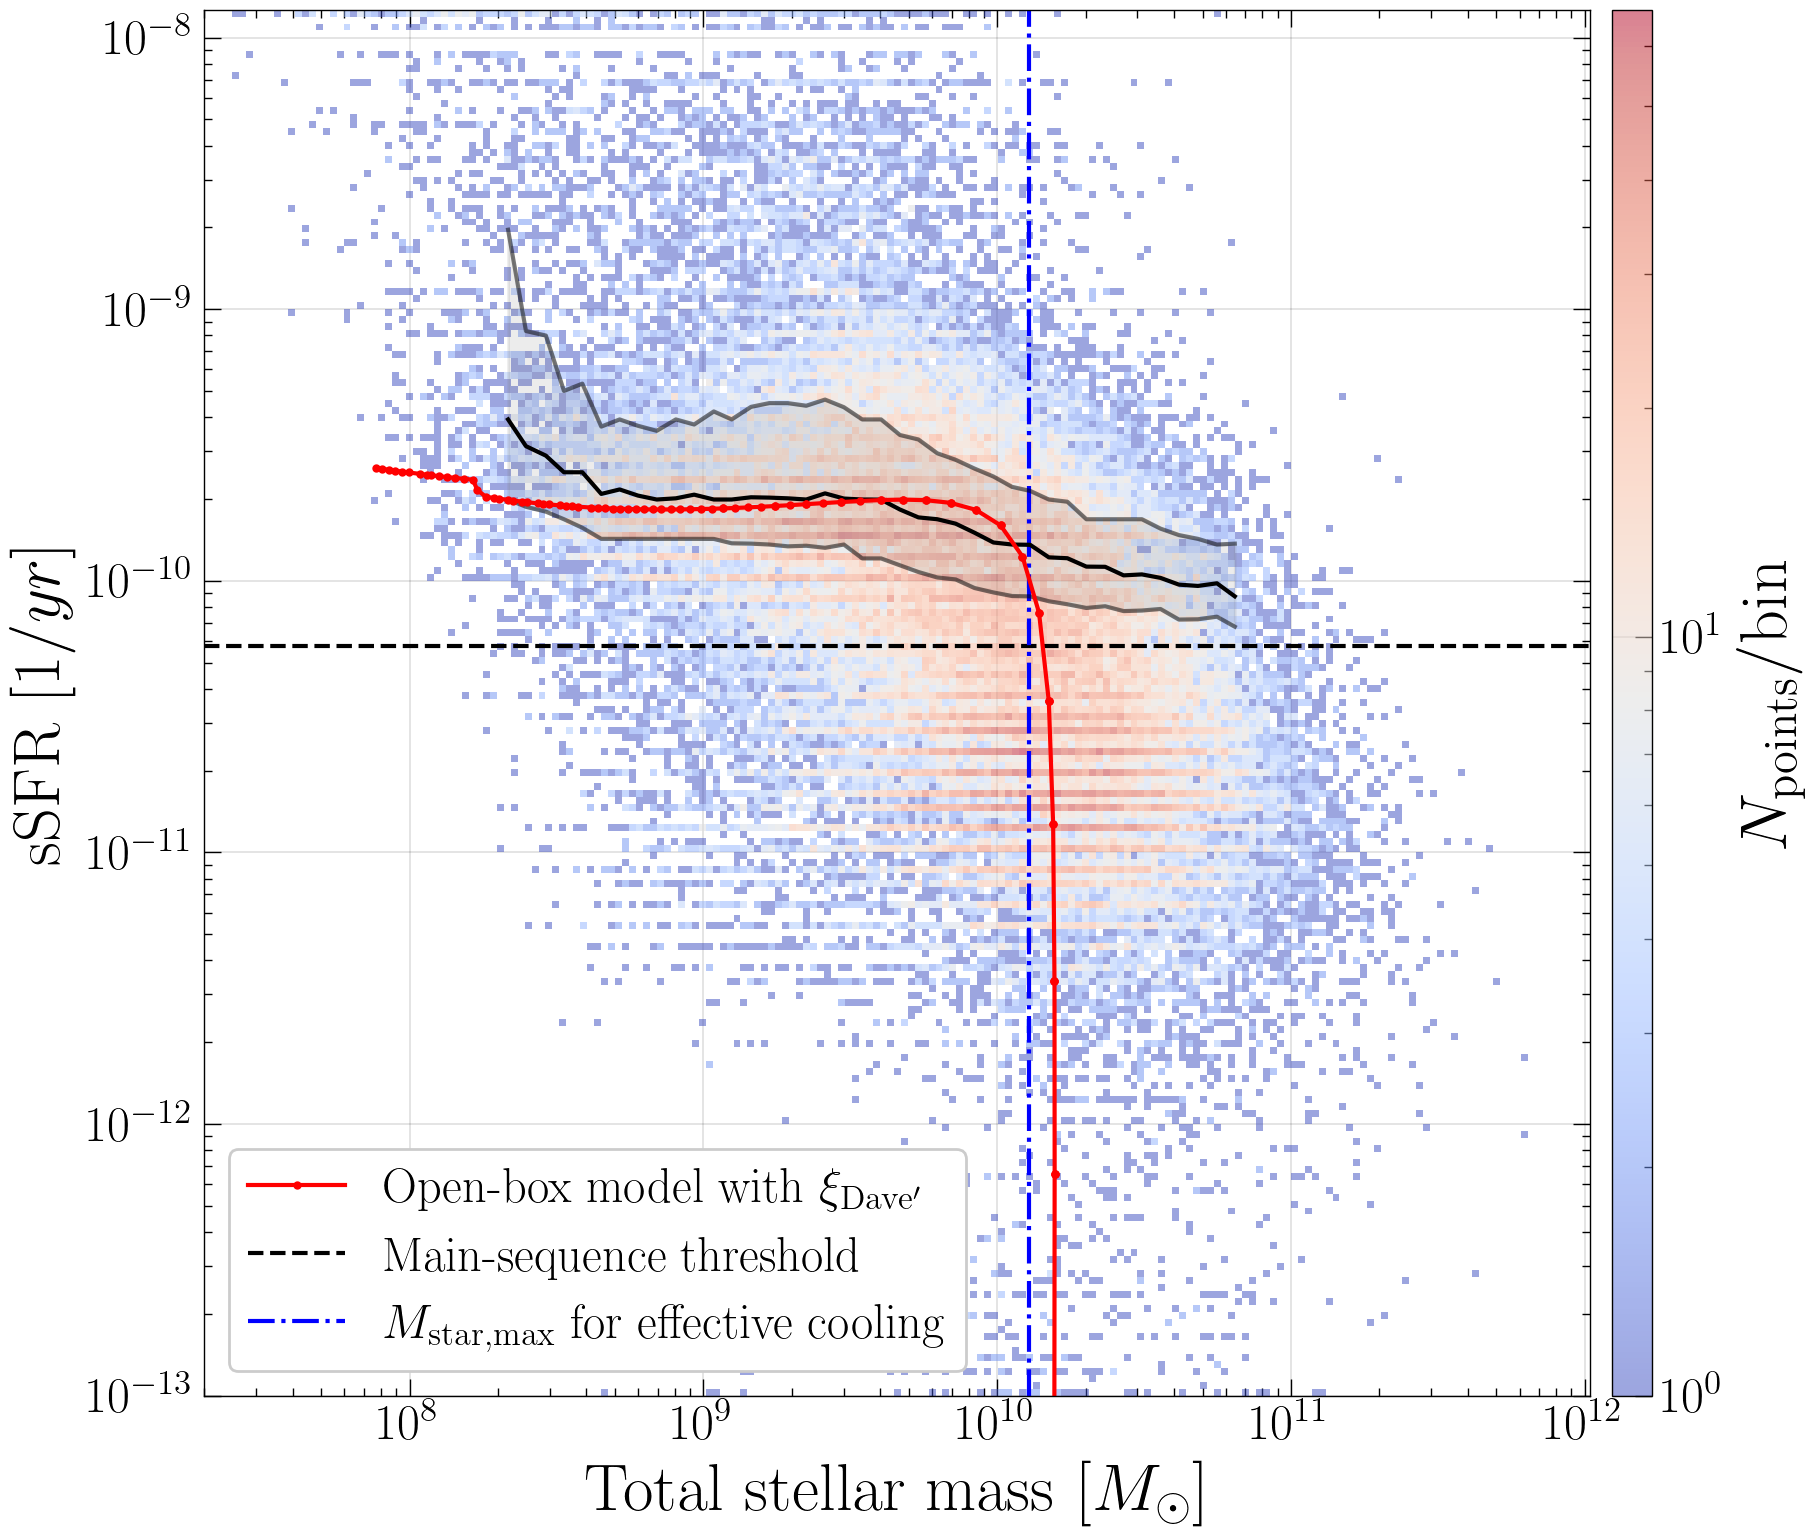
\includegraphics[width=\columnwidth]{openbox_dave.png}
    \caption{The main panel shows a 2D histogram of sSFR versus $M_{\text{star}}$ for our dataset. The side panels display the marginal distributions of the two axes. The black dashed line indicates the value where the sSFR distribution has a local minimum, which is used to separate the main sequence from quiescent galaxies. The 2D Gaussian contours of the two populations are also shown.}
    \label{fig:openbox_dave}
\end{figure}
%%%%%%%%%%%%%%%%%%%%%%%%%%%%%%%%%%%%%%%%%%%%%%%%%%



\section{Discussion}\label{sec:discussion}

%%%%%%%%%%%%%%%%%%%%%%%%%%%%%%%%%%%%%%%%%%%%%%%%%%



\section{Summary}\label{sec:summary}

%%%%%%%%%%%%%%%%%%%%%%%%%%%%%%%%%%%%%%%%%%%%%%%%%%%%%%%%%%%%%%%%%%%%%%%%%%%%%%%%%%%%%%%%%%%%%%%%%%%%




%%%%%%%%%%%%%%%%%%%% REFERENCES %%%%%%%%%%%%%%%%%%%%%%%%%%%%%%%%%%%%%%%%%%%%%%%%%%%%%%%%%%%%%%%%%%%%
% The best way to enter references is to use BibTeX:
\bibliographystyle{mnras}
\bibliography{bibliography} 
%%%%%%%%%%%%%%%%%%%%%%%%%%%%%%%%%%%%%%%%%%%%%%%%%%%%%%%%%%%%%%%%%%%%%%%%%%%%%%%%%%%%%%%%%%%%%%%%%%%%


% Don't change these lines
\label{lastpage}
\end{document}
